\chapter{Analyzing the Single Shot Detector}


Our goal is to improve SSD detector proposed by \citeauthor{bib:ssd} and adjust it to fit the needs of video surveillance.  

Because we use another framework and have access to different hardware than the one used in SSD research paper, we can not compare our performance results with the reported values. Similarly, SSD's precision is heavily dependent on the training dataset and therefore on the data augmentation process. The augmentation we used in our experiments proved to be inferior to the original ones, and our precision values are therefore lower. However, we do not mind those problems, because we trained our version of SSD which we can use as a baseline for our comparisons. 





\section{Base network}
Our goal is to find the best possible architecture of SSD-like network that can be later improved by expanding the dataset and hyper-parameter tuning. We started by implementing the SSD detector on multiple base networks and training them on COCO dataset. We recognize that the SSD is based upon relatively old VGG-16 network that lacks in both speed and precision compared to more modern CNNs. Because the base network serves as a feature extractor, upon which SSD performs detection, it is the integral part of the network and we believe that has a large impact on overall performance. 

\subsection{Architectures}
We decided to try to implement SSD on three 'post-VGG' networks, namely \textit{ResNet}, \textit{Xception} and \textit{NASNet}. We choose ResNet because it is a well-known network with simple design and easy scalability. Xception got our attention for its performance as a classification network in \citeauthor{bib:cnnbenchmark} benchmark (\cref{sec:cnncomp}) taking a middle ground between speed and precision. NASNet, or precisely NASNet-A-Mobile, was chosen out of curiosity for its unique structure compared to the other two networks. We will be referring to ResNet networks by their number of layers, e.g., ResNet50. Also, Xception will be called Xception version A, or shortly XceptionA, to avoid confusion with a version we are going to introduce later.

First of all, we needed to decide how to connect the detection layers of SSD to our base networks. SSD uses six feature layers, two extracted from the VGG-16 network and four from extra layers. The feature sizes are: [38\x38\x512], [19\x19\x1024], [10\x10\x512], [5\x5\x256], [3\x3\x256] and [1\x1\x256] for input image of 300\x300 pixels. We decided to copy the spatial resolution of feature layers as closely as possible without changing the structure of tested base networks. That means we have not kept the number of channels equal to SSD's. However, not enough channels could impact the SSD's precision, and too many channels will surely have an impact on the detection speed.

Our general strategy was to find the deepest layer with size as close as possible for every VGG's feature and then add the extra layers as needed. We copied the same set of extra layers from SSD on VGG-16, with the pair of two convolution layers for each feature map. One 1\x1 convolution for channel reduction, and one 3\x3 convolution for feature generation. The final feature sizes are listed in \cref{tab:features}. Each feature map is then fed into both classification and localization layer for the corresponding scale, as described in \cref{fig:VGGSSD}.

\begin{table}
    \centering
    \begin{tabular}{c|c|c|c|c}
        VGG-16 & ResNet34 & ResNet50/101 & XceptionA & NASNet* \\ 
        \hline
        38\x 512 &   38\x 128 &  38\x 512 &     37\x 256 &  28\x 264\\
        19\x 1024 &  19\x 256 &  19\x 1024 &    19\x 728 &  14\x 528\\
        10\x 512 &   10\x 512 &  10\x 2048 &    10\x 2048 & 7\x 1056\\
        5\x 256 &    5\x 512 &   5\x 512 &      5\x 512 &   4\x 512\\
        3\x 256 &    3\x 256 &   3\x 256 &      3\x 256 &   2\x 256\\
        1\x 256 &    1\x 256 &   1\x 256 &      1\x 256 &\\
    \end{tabular}
    \caption[Feature sizes of SSD's base networks]{Sizes of feature maps used in SSD's detection. The sizes are calculated for input image of 300\x300 pixels, with the exception of NASNet, which only works on 224\x224 inputs. First number is spacial dimension of square feature and the second one represents the number of channels.}
    \label{tab:features}
\end{table}

\paragraph{ResNet} We had a bit of luck finding the right layers for feature extraction in ResNet networks. The high-level \textit{Layers} in ResNet produce features of 75\x75, 38\x38, 19\x19 and 10\x10 sizes. We simply picked the outputs of second, third and fourth layers and added appropriate feature layers after last \textit{Layer} for the rest of the features. The spatial dimensions of feature sizes are consistent on all ResNet version, with the only difference being the depth of the channels. The architecture of ResNet-SSD, with highlighted detection feature maps is illustrated on \cref{fig:resnet_xception_SSD}.

\paragraph{XceptionA} The high-level architecture of Xception, the entry, middle and exit flow, produce the features of 19\x19, 19\x19 and 10\x10 sizes. We can use the latter two outputs, but we had to step deeper into the entry flow and get the 38\x38 feature from the second block of the network. The network is topped by adding six extra layers that provide the remaining three feature maps. The XceptionA-SDD is illustrated on \cref{fig:resnet_xception_SSD}.


\begin{figure}
    \centering
    \resnetSSD
    \caption[Resnet34-SSD and Xception-SSD]%
    {Resnet34-SSD(left) and XceptionA-SSD (right). For details on \textit{Layers} and \textit{Blocks} see \cref{fig:resnet_arch} and \cref{fig:xception} respectively. Extra layers are highlighted with a red dashed rectangle.}

    \label{fig:resnet_xception_SSD}
\end{figure}

\paragraph{NASNet} The architecture of NASNet has proven to be the trickiest one for implementing SSD. Even though it is a fully convolutional network, due to the complex structure with many additions and concatenations, it does not accept any input except for 224\x224 pixels. Rather than doing large scale changes to the architecture, we decided to compromise on the detector side and use the lower resolution. 

Other than the input size, the next problem of the NASNet-A-Mobile is the lack of choice of feature maps for detection. Because the stacks of Normal Cells do not change the spatial dimensions, there are only three available sizes of feature maps. Without any real choice, we end up with features of 28\x28, 14\x14 and 7\x7 sizes. The problem here is that 7\x7 feature map has only enough pixels for two subsequent 3\x3 convolutions. Therefore we had to implement SSD with only five feature layers for detections. See \cref{fig:nasnetSSD} for architecture details.


\begin{figure}
    \centering
    \nasnetSSD
    \caption[NASNet-SSD]%
    {NASNet-SSD based on NASNet-A-Mobile. The network is limited to input of size 224\x224 due to complex structure of NASNet cells. For detailed description of cells see \cref{sec:nasnet}.}
    \label{fig:nasnetSSD}
\end{figure}

\subsection{Performance results}
We trained the SSDs on COCO dataset, to compare their performance, both in terms of precision and speed. The base networks we choose to compare are VGG-16, ResNet34, ResNet50, ResNet101, XceptionA, and NASNet-A-Mobile. For a relevant comparison, all networks were implemented in the same framework and trained for an equal number of iterations. We can see, from the results in \cref{fig:cocoperf}, that VGG-16 is outperformed by all of our choices in terms of speed, but overcomes the XceptionA and NASNet in precision. 

We believe that the compromises we had to make in implementing NASNet-SSD, the smaller input image resolution, fewer feature maps for detections, are the reason for the poor precision performance. Concerning XceptionA, we hypothesize that we extract the first feature map from a too shallow layer, after passing only six convolutional layers. If the first feature map is compromised, that would impact the detection of small objects and have a substantial impact on the precision. We will test our hypothesis and try to rectify the problem of Xception-SSD in \cref{sec:fixxception}.

\begin{figure}
    \centering
    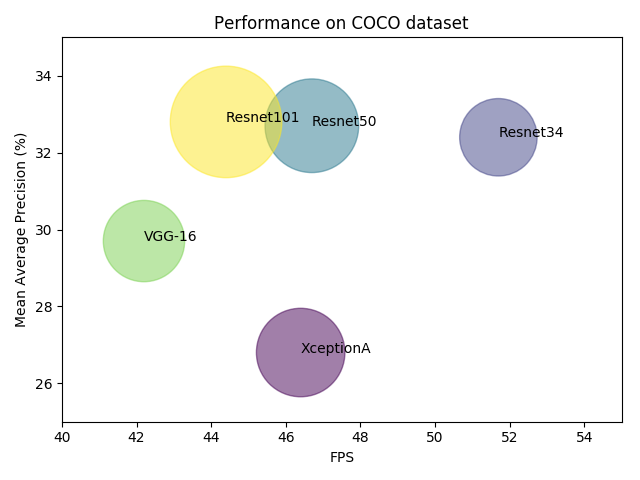
\includegraphics[width=\textwidth]{img/coco_perf}
    \caption[Performance of SSD base networks on COCO dataset]{Performance of SSD detector on multiple base networks. Circle diameters demonstrate relative difference of network parameter counts.}
    \label{fig:cocoperf}
\end{figure}

\section{Training data and classes}
The main problem of solving problems with neural networks, is the lack of available data. Some problems can be solved by reinforcement learning, but others, like the object detection, need supervision. Creating a custom, problem specific, dataset requires a lot of manpower and is viable only for big companies. Therefore, dependent on public datasets like COCO. The problem of such datasets is that they often include many classes that are not needed for certain application. For surveillance we are interested in classes such as people and vehicles. We are going to compare the performance and precision of SSDs between training on full COCO dataset and a subset for surveillance. We expect significant performance improvement with lowering the number of detector classes, however we were not sure how will this chance impact performance. 

\paragraph{Surveillance dataset classes}
\begin{multicols}{2}
    \begin{itemize}
        \item person
        \item bicycle
        \item motorcycle
        \item car
        \item bus
        \item truck
        \item train
    \end{itemize}
\end{multicols}

\subsection{Precision impact}
Training a network on a subset of larger dataset seems to be a straightforward task. However, we hypothesize that by removing of classes with similar features to the ones we are detecting, there is a possibility of increasing the error on those selected classes. 

For example, consider a dataset of humans and monkeys. The networks learns to distinguish between the two and classifies everything else as a background. If we do not care about monkeys, we can simply filter them out in post-processing. However, consider a network that is trained to only recognize people and use it on a monkey. We are worried that such network would classify a monkey as a person, based on a large number of similar features. 

To counter-measure the possibility of larger amount of false positives, we decided to increase the amount of negative samples. We did it by only filtering annotation from \textit{COCO} dataset to create the \textit{surveillance dataset}, but keeping all the images, even those without positive ground-truths. The expectation is to reach similar precision on selected classes, on both \textit{COCO} and \textit{surveillance dataset}. However, because \textit{COCO} is small dataset with only about hundred thousand images and is certainly not exhaustive in classes with similar features to \textit{surveillance dataset}, this measure would only help on our evaluation data.

\paragraph{Results} in \cref{tab:ssdcocosurv} show that it is possible to remove unnecessary classes from the dataset without impacting the performance. We tested the approach on multiple architectures, and the results do not conclusively favor one dataset over the other. 

\begin{table}[]
    \centering
    \begin{tabular}{c|c|c}
         & COCO & Surveillance  \\
         \hline
        ResNet34 & 47.3 & 47.3 \\
        ResNet50 & 46.6 & 48.7 \\
        ResNet101 & 47.2 & 45.7 \\
        XceptionA & 39.4 & 37.8 \\
        NASNet & & 36.9 
    \end{tabular}
    \caption[SSD's precision comparison between COCO and surveillance datasets]{Mean average precision of \textit{surveillance} classes. Comparing networks trained on all 80 classes of \textit{COCO} dataset and \textit{surveillance} subset of \textit{COCO}.}
    \label{tab:ssdcocosurv}
\end{table}
\todo{nasnet data}

\subsection{Performance impact}
We expect proportional increase of performance with removal of the classes. We saw that in the SSD (\cref{fig:VGGSSD}) the depth of the classification layers is dependent on the number of classes. Another important factor is that smaller dimensions of detection tensors will result in faster post-processing, i.e., non-maximum suppression. 

We illustrate the effect of number of detected classes on performance on \cref{fig:fpscls}, based on measured data. Although the relationship of frames per second and classes is hyperbolic, on the interval between 7 and 80 classes, we approximate the loss of 0.78 frames per second per class on ResNet50-SSD. This is a significant number and means that training the networks for special purposes can bring a large benefit as opposed to using a general detector for everything.

\begin{figure}
    \centering
    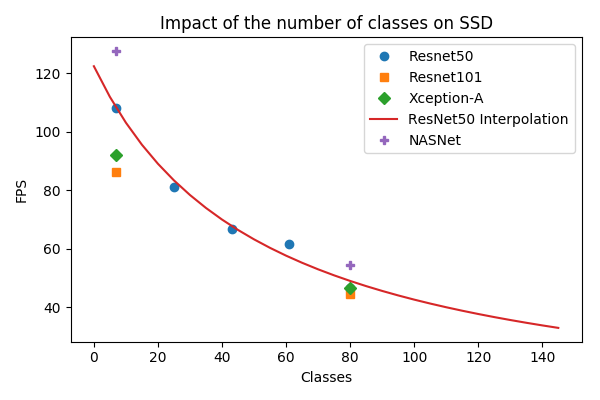
\includegraphics[width=\textwidth]{img/fps_class}
    \caption[Impact of the number of classes on SSD performance]{Impact of the number of classes on SSD performance. Inference time values (1/fps) are linearly interpolated, the result is therefore hyperbolic approximation of frames per second.}
    \label{fig:fpscls}
\end{figure}
\todo{add NASNet data}


\section{Modifying Xception}
\label{sec:fixxception}



\section{SSD-TC: SSD with temporal convolution}
\begin{figure}
    \centering
    \ssdtc
    \caption[SSDTC architecture]{SSDTC architecture on ResNet34 base. stride 1, no padding in the dimension of stacked features therefore no detections for first and last two images, therefore efficiency grows with bigger chunks}
    \label{fig:ssdtc}
\end{figure}


HHEADS SSD: 80.5\%

SSDTC (3): 78.7\%

SSDTC(5): x\%
